\documentclass[10pt,a4paper]{article}

% ---------- page, fonts, spacing ----------
\usepackage[a4paper,top=2.0cm,bottom=2.1cm,left=2.2cm,right=2.2cm]{geometry}
\usepackage[T1]{fontenc}
\usepackage{newtxtext,newtxmath}          % Times-style text and maths
\usepackage[final]{microtype}
\usepackage{setspace}
\setstretch{1.03}
\emergencystretch=1.5em
\setlength{\parindent}{0pt}
\setlength{\parskip}{3pt plus 1pt}

% ---------- floats, tables, captions ----------
\usepackage{graphicx}
\usepackage{booktabs}
\usepackage{array}
\usepackage[font=small,labelfont=bf,labelsep=period,skip=3pt]{caption}
\usepackage{subcaption}
\setlength{\textfloatsep}{8pt plus 2pt minus 2pt}
\setlength{\floatsep}{6pt plus 2pt minus 2pt}
\setlength{\intextsep}{6pt plus 2pt minus 2pt}
\graphicspath{{../figures/}}
\renewcommand{\topfraction}{0.9}
\renewcommand{\bottomfraction}{0.8}
\renewcommand{\textfraction}{0.07}
\renewcommand{\floatpagefraction}{0.85}
\setcounter{topnumber}{3}
\setcounter{totalnumber}{5}

% ---------- headings ----------
\usepackage{titlesec}
\titleformat{\section}{\normalfont\large\bfseries}{\thesection}{0.6em}{}
\titleformat{\subsection}{\normalfont\normalsize\bfseries}{\thesubsection}{0.6em}{}
\titlespacing*{\section}{0pt}{8pt plus 2pt minus 2pt}{2pt}
\titlespacing*{\subsection}{0pt}{5pt plus 1pt minus 1pt}{0pt}

\usepackage{amsmath}
\usepackage[hidelinks]{hyperref}
\usepackage{enumitem}
\setlist{nosep,leftmargin=1.4em,topsep=1pt}

\newcommand{\code}[1]{\texttt{\small #1}}

\begin{document}

% ---------- title block ----------
\begin{center}
{\LARGE\bfseries Classification of Countries into HDI-Based Development\\[3pt] Categories Using World Bank Indicators\par}
\vspace{7pt}
{\large DS203 Course Project, Classification Track\par}
\vspace{7pt}
\begin{tabular}{ccc}
Tanish Jain & Ruturva Vaghasia & Arnav Jain\\
\small 25B4244 & \small 25B4205 & \small 25B2704
\end{tabular}\par
\vspace{3pt}
{\small November 2026 \quad$\cdot$\quad Code and data: \url{https://github.com/tanishjain0911-beep/ds203-hdi-classification}\par}
\end{center}

\section{Introduction}
The Human Development Index (HDI) published by UNDP combines life expectancy, education and income into one score
between 0 and 1. It depends on survey and census data, so it appears one to two years late. The World Bank reports
economic, infrastructure and health indicators for almost every country each year. We ask whether these routinely
available indicators are enough to place a country in the correct development category, and which of them carry
the most information.

We build the target from the 2023 HDI score: \textbf{Low} ($\text{HDI} < 0.550$), \textbf{Medium/High}
($0.550 \le \text{HDI} < 0.800$) and \textbf{Very High} ($\text{HDI} \ge 0.800$). This three-class grouping is
defined for the project; UNDP's official scheme has four categories. To avoid target leakage, the HDI score and its
components (life expectancy, expected and mean years of schooling, GNI per capita) are not used as predictors, and
country names and ISO codes are identifiers only. We compare four classifiers, test whether the categorical
features and PCA improve them, and treat every result as a predictive association, not a causal effect.

\section{Methodology}
\subsection{Data sources and country matching}
The target is the column \code{hdi\_2023} of the UNDP Human Development Report 2025 release (\emph{composite
indices complete time series}, accessed 23 November 2026). The nine predictors in Table~\ref{tab:data} are World
Development Indicators, downloaded as one CSV file per indicator from the World Bank data portal on 25 November
2026. Region comes from the country metadata file in the same download; aggregates such as world, regional and
income-group totals have no region and were removed.

We merged the tables on ISO3 codes. All 195 UNDP countries matched, so no code had to be corrected by hand. The 22
World Bank economies without an HDI, mostly territories such as Puerto Rico and Greenland, were left out, and
Monaco and DPR Korea were dropped because they have no 2023 HDI. The final dataset has 193 countries: 26 Low
(13.5\%), 93 Medium/High (48.2\%) and 74 Very High (38.3\%).

\begin{table}[!htb]
\centering\small
\begin{tabular}{llrrrr}
\toprule
 & & & \multicolumn{3}{c}{Median by class}\\
\cmidrule(lr){4-6}
Indicator & WDI code & Missing (\%) & Low & Med./High & Very High\\
\midrule
GDP growth (annual \%) & \code{NY.GDP.MKTP.KD.ZG} & 2.1 & 4.3 & 3.5 & 2.0\\
Inflation, consumer prices (annual \%) & \code{FP.CPI.TOTL.ZG} & 7.8 & 7.5 & 6.0 & 5.0\\
Unemployment (\% of labour force) & \code{SL.UEM.TOTL.ZS} & 7.3 & 4.7 & 5.4 & 5.2\\
Infant mortality (per 1{,}000 births) & \code{SP.DYN.IMRT.IN} & 1.0 & 45.7 & 17.7 & 4.0\\
Access to electricity (\% of pop.) & \code{EG.ELC.ACCS.ZS} & 0.0 & 45.4 & 99.3 & 100.0\\
Internet users (\% of pop.) & \code{IT.NET.USER.ZS} & 5.7 & 23.7 & 69.6 & 92.2\\
Agriculture value added (\% of GDP) & \code{NV.AGR.TOTL.ZS} & 3.6 & 29.0 & 10.3 & 2.1\\
Industry value added (\% of GDP) & \code{NV.IND.TOTL.ZS} & 3.6 & 22.2 & 26.3 & 23.7\\
Trade (\% of GDP) & \code{NE.TRD.GNFS.ZS} & 11.9 & 55.3 & 75.0 & 107.3\\
\bottomrule
\end{tabular}
\caption{The nine World Bank predictors: share of the 193 countries with a missing value, and the median in each
HDI class. Region (7 levels, complete) and \code{DominantSector} (3.6\% missing) are the categorical predictors.}
\label{tab:data}
\end{table}

\subsection{Reference year and engineered feature}
Every indicator takes its 2023 value. When that is missing we use the 2022 value, then the 2021 value, and never a
year after 2023. The dataset records the year of every value; 19 of the 1{,}737 predictor values come from 2021 or
2022. Values still missing after this step stay missing for the imputation experiments.

\code{DominantSector} is the largest of the agriculture, industry and services shares, with services estimated as
$100 - \text{agriculture} - \text{industry}$. It is set to missing when a share is missing or negative. Services is
the largest share in 176 countries, industry in 8 oil and mining economies such as Qatar, Kuwait and Libya, and
agriculture in Niger and Chad; 7 countries have no value.

\subsection{Outliers and transformations}
Inflation and trade are strongly right-skewed. Inflation has 19 values above the upper IQR fence of about 18\%, led
by Lebanon (221\%), Sudan (139\%) and Argentina (133\%), and trade reaches 403\% of GDP in Luxembourg and 353\% in
Hong Kong. These are real values, and no percentage variable falls outside the range 0 to 100, so we kept every
observation. Both features are transformed with $\operatorname{sign}(x)\ln(1+|x|)$, which also handles the
negative inflation values. The formula has no learned parameters, so applying it before the split does not leak
information.

\subsection{Split and preprocessing}
The observations are countries, not a time series, so we use a stratified 60/20/20 split with
\code{random\_state=42}: 115 training, 39 validation and 39 test countries, of which 16, 5 and 5 are Low. All
learned preprocessing sits in a scikit-learn \code{Pipeline} built around a \code{ColumnTransformer}, so it is
fitted on training data only and refitted inside every cross-validation fold. Numerical features are imputed with
the training mean (chosen in Section~\ref{sec:imp}) and standardised. Categorical features get an explicit
``Missing'' level and are one-hot encoded with \code{handle\_unknown="ignore"}, giving 20 model inputs in total.

\subsection{Models, tuning and evaluation}
We train a majority-class baseline and three models, tuned with \code{GridSearchCV} on stratified 5-fold
cross-validation of the training set:
\begin{itemize}
\item multinomial logistic regression with an L2 penalty (\code{max\_iter=5000}), $C \in \{0.01, 0.1, 1, 10, 100\}$;
\item a decision tree, maximum depth $\in \{2, 3, 4, 5, \text{none}\}$, minimum leaf size $\in \{1, 3, 5\}$;
\item a random forest of 300 trees, maximum depth $\in \{3, 5, \text{none}\}$, minimum leaf size $\in \{1, 3\}$.
\end{itemize}
The selection criterion is macro F1, which weights the small Low class equally with the other two. The imputation,
PCA and feature-set comparisons use the same folds with default model settings and were made before tuning. We use
the validation set only to compare the tuned models, then refit each model on training plus validation data (154
countries) and evaluate it once on the test set with accuracy, balanced accuracy, macro F1, per-class F1 and a
confusion matrix. The test set plays no part in any modelling decision.

\section{Experiments}
\subsection{Missing data}
Trade is the most incomplete indicator (11.9\% missing), followed by inflation (7.8\%) and unemployment (7.3\%);
electricity access and region are complete (Figure~\ref{fig:missing}). Gaps are concentrated in the least developed
countries: 35\% of Low countries have at least one missing indicator, against 27\% of Medium/High and 12\% of
Very High countries, and a Low country has 1.12 missing values on average against 0.22 for a Very High country.
Unemployment is the exception, with no gaps in the Low class. The most incomplete records belong to
conflict-affected countries (Eritrea, Yemen, South Sudan, Somalia) and to very small states (Tuvalu, Nauru). The
data are therefore not missing at random, and imputed values for Low countries come largely from richer countries.

\begin{figure}[!htb]
\centering
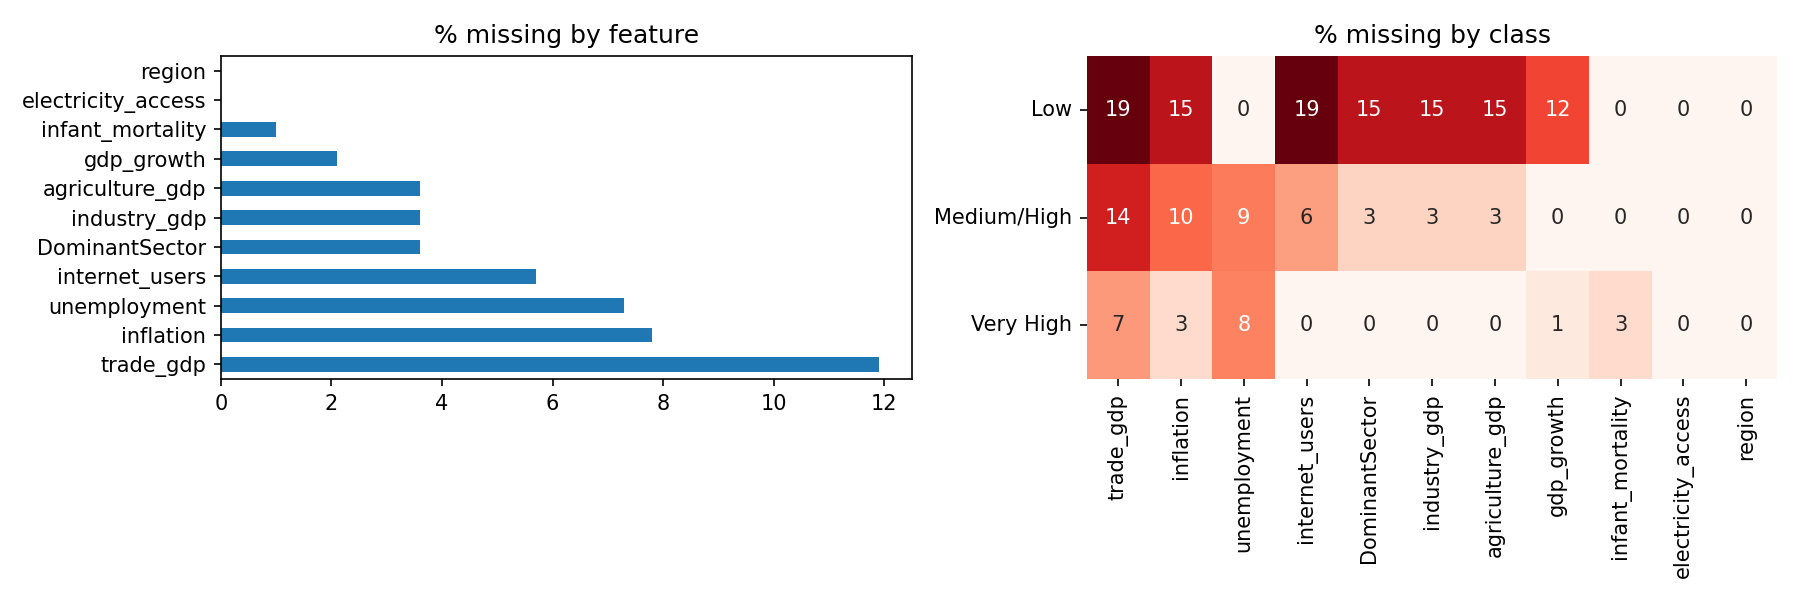
\includegraphics[width=0.72\textwidth]{missingness.png}
\caption{Share of missing values by feature (left) and within each HDI class (right), in percent.}
\label{fig:missing}
\end{figure}

\subsection{Indicators across classes}
Infant mortality, electricity access, internet use and the agriculture share change steadily from Low to Very High
(Table~\ref{tab:data}). Median infant mortality falls from 45.7 to 4.0 per 1{,}000 births and median internet use
rises from 24\% to 92\%. Trade is higher in Very High countries, GDP growth is slightly higher in Low countries, and
unemployment and the industry share show no clear order. The same four indicators are strongly correlated with
each other: all six pairs with $|r| \ge 0.5$ come from this group, the strongest being electricity and internet
($r = 0.84$) and infant mortality and internet ($-0.83$). They largely measure one underlying level of development.

Region is also related to the class: 22 of the 26 Low countries are in Sub-Saharan Africa and the other 4 in the
Middle East \& North Africa, 44 of the 51 countries in Europe \& Central Asia are Very High, and all six South Asian
countries are Medium/High.

\subsection{Imputation and missingness indicators}\label{sec:imp}
Mean imputation without missingness indicators gave the best cross-validated macro F1 for logistic regression
($0.839 \pm 0.068$) and for the random forest ($0.890 \pm 0.061$). Median imputation scored 0.818 and 0.875. A
missingness indicator is a 0/1 column that marks an imputed value, so a model can use the fact that a country did
not report it. Given the pattern above this could help, but the indicators lowered macro F1 to 0.797 and 0.881,
probably because the extra columns are almost all zeros and add noise with only 115 training countries. All
differences are within one standard deviation, and we use mean imputation without indicators.

\subsection{Principal component analysis}
We fitted PCA to the preprocessed training features (Figure~\ref{fig:pca}). The first component explains 38.8\% of
the variance, and seven of the 20 components are needed to reach 90\%. PC1 is a development axis, with loadings on
internet use ($+0.48$), electricity ($+0.46$), infant mortality ($-0.46$) and agriculture share ($-0.45$). PC2
mostly reflects short-run conditions (GDP growth $+0.69$, inflation $-0.41$). Along PC1 the Low class separates
clearly, while Medium/High and Very High overlap.

Keeping two or three components raised the cross-validated macro F1 of logistic regression to 0.857, within one
standard deviation of the model without PCA. Every PCA setting lowered the random forest (0.82 to 0.87 against
0.890), since its trees split best on the original features. The final models do not use PCA, which also keeps
them interpretable.

\begin{figure}[!htb]
\centering
\begin{subfigure}[b]{0.42\textwidth}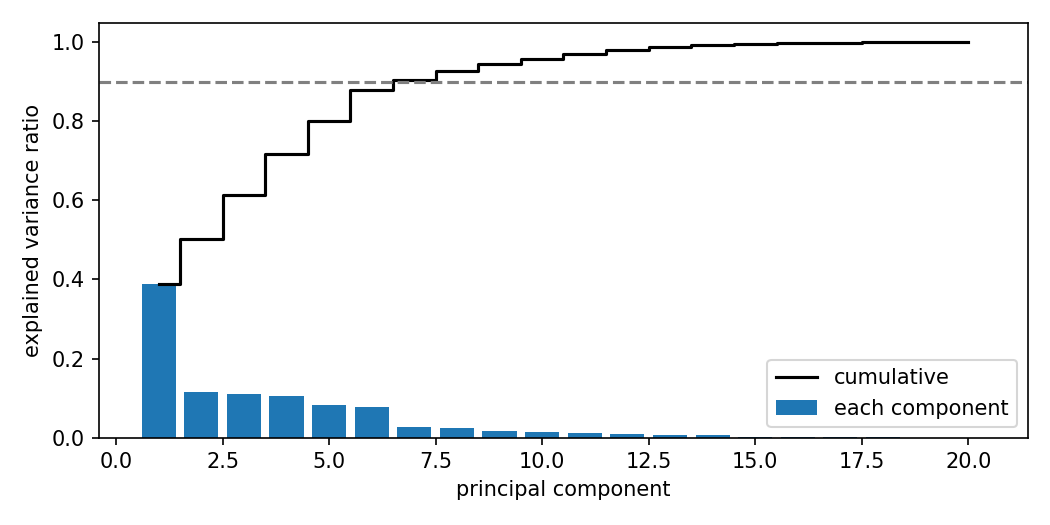
\includegraphics[width=\linewidth]{pca_explained_variance.png}\end{subfigure}\hspace{0.04\textwidth}
\begin{subfigure}[b]{0.34\textwidth}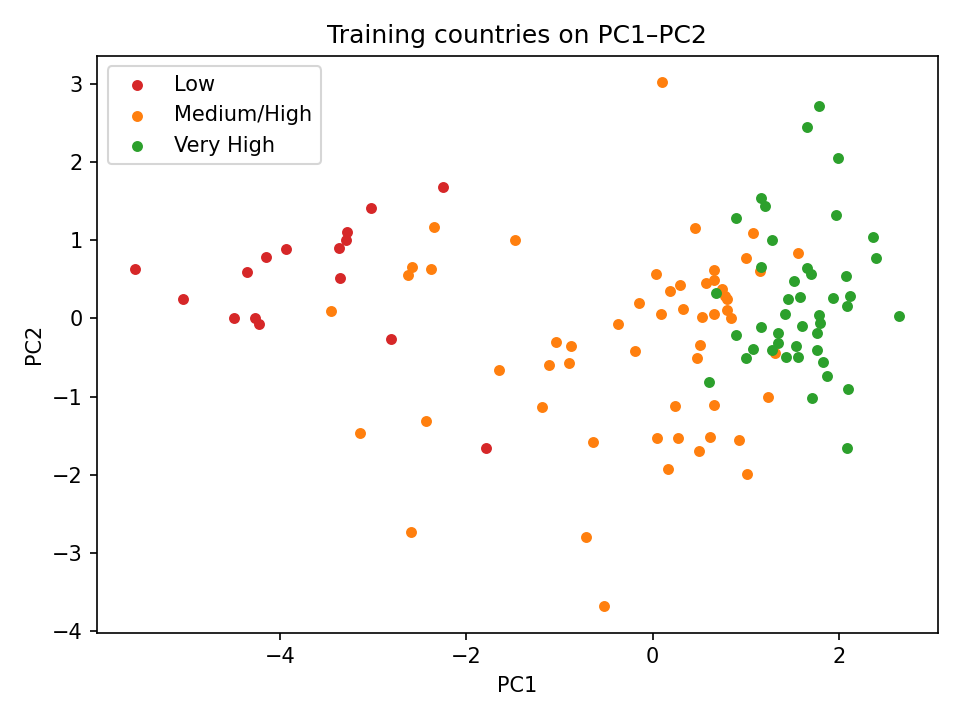
\includegraphics[width=\linewidth]{pca_scatter.png}\end{subfigure}
\caption{PCA of the preprocessed training features. Left: explained variance ratio per component and cumulative
total. Right: training countries on the first two components.}
\label{fig:pca}
\end{figure}

\subsection{Numerical and categorical features}
The numerical indicators carry almost all of the signal (Table~\ref{tab:features}). Region and
\code{DominantSector} alone reach a macro F1 of about 0.5, mainly because region picks out Sub-Saharan Africa.
Adding either one to the numerical features changes macro F1 by at most 0.01, so neither improves prediction in a
meaningful way. For the sector this is expected: it is ``Services'' for 91\% of countries and is computed from
shares the model already has. We keep the combined set, since the differences are within $\pm 0.01$ and it lets us
discuss region.

\begin{table}[!htb]
\centering\small
\begin{tabular}{lcc}
\toprule
Feature set & Logistic regression & Random forest\\
\midrule
Numerical only & 0.846 & 0.888\\
Categorical only (region and sector) & 0.512 & 0.545\\
Numerical and region & 0.837 & 0.890\\
Numerical and \code{DominantSector} & 0.846 & 0.895\\
All features & 0.839 & 0.890\\
\bottomrule
\end{tabular}
\caption{Cross-validated macro F1 for different feature sets (training set, five folds).}
\label{tab:features}
\end{table}

\subsection{Model selection}
All three models are far above the baseline (Table~\ref{tab:cv}). The random forest has the highest
cross-validated macro F1, but its lead over logistic regression (0.046) is smaller than the standard deviation
across folds, and logistic regression is slightly ahead on the validation set. Each fold holds about 23 countries,
only three or four of them Low, so the ranking of these two models is uncertain. Logistic regression selected
$C = 100$, the weakest regularisation in the grid, which makes it close to an unregularised model.

\begin{table}[!htb]
\centering\small
\begin{tabular}{lccl}
\toprule
Model & CV macro F1 & Validation macro F1 & Selected hyperparameters\\
\midrule
Majority baseline & $0.216 \pm 0.000$ & 0.218 & predicts Medium/High\\
Logistic regression & $0.849 \pm 0.094$ & 0.799 & $C = 100$\\
Decision tree & $0.801 \pm 0.071$ & 0.703 & max.\ depth 4, min.\ leaf 3\\
Random forest & $0.895 \pm 0.074$ & 0.784 & max.\ depth 5, min.\ leaf 1\\
\bottomrule
\end{tabular}
\caption{Macro F1 in 5-fold cross-validation on the training set (mean $\pm$ standard deviation) and on the
validation set.}
\label{tab:cv}
\end{table}

\subsection{Test-set results}
Logistic regression has the best test macro F1 and balanced accuracy (both 0.708), and the random forest the best
accuracy (0.821) with an almost perfect Very High class (F1 0.97), as Table~\ref{tab:test} shows. Recall on the
Low class is poor. Logistic regression finds two of the five Low test countries, the forest one and the tree none.
One country is worth 2.6 percentage points of accuracy, so the test ranking depends on a few countries, and all
test scores are below the cross-validation estimates.

\begin{table}[!htb]
\centering\small
\begin{tabular}{lcccccc}
\toprule
 & & Balanced & Macro & \multicolumn{3}{c}{F1 by class}\\
\cmidrule(lr){5-7}
Model & Accuracy & accuracy & F1 & Low & Medium/High & Very High\\
\midrule
Majority baseline & 0.487 & 0.333 & 0.218 & 0.00 & 0.66 & 0.00\\
Logistic regression & 0.795 & \textbf{0.708} & \textbf{0.708} & 0.40 & 0.79 & 0.93\\
Decision tree & 0.667 & 0.512 & 0.497 & 0.00 & 0.72 & 0.77\\
Random forest & \textbf{0.821} & 0.676 & 0.682 & 0.25 & 0.83 & 0.97\\
\bottomrule
\end{tabular}
\caption{Results on the 39 held-out test countries (5 Low, 19 Medium/High, 15 Very High).}
\label{tab:test}
\end{table}

\begin{figure}[!htb]
\centering
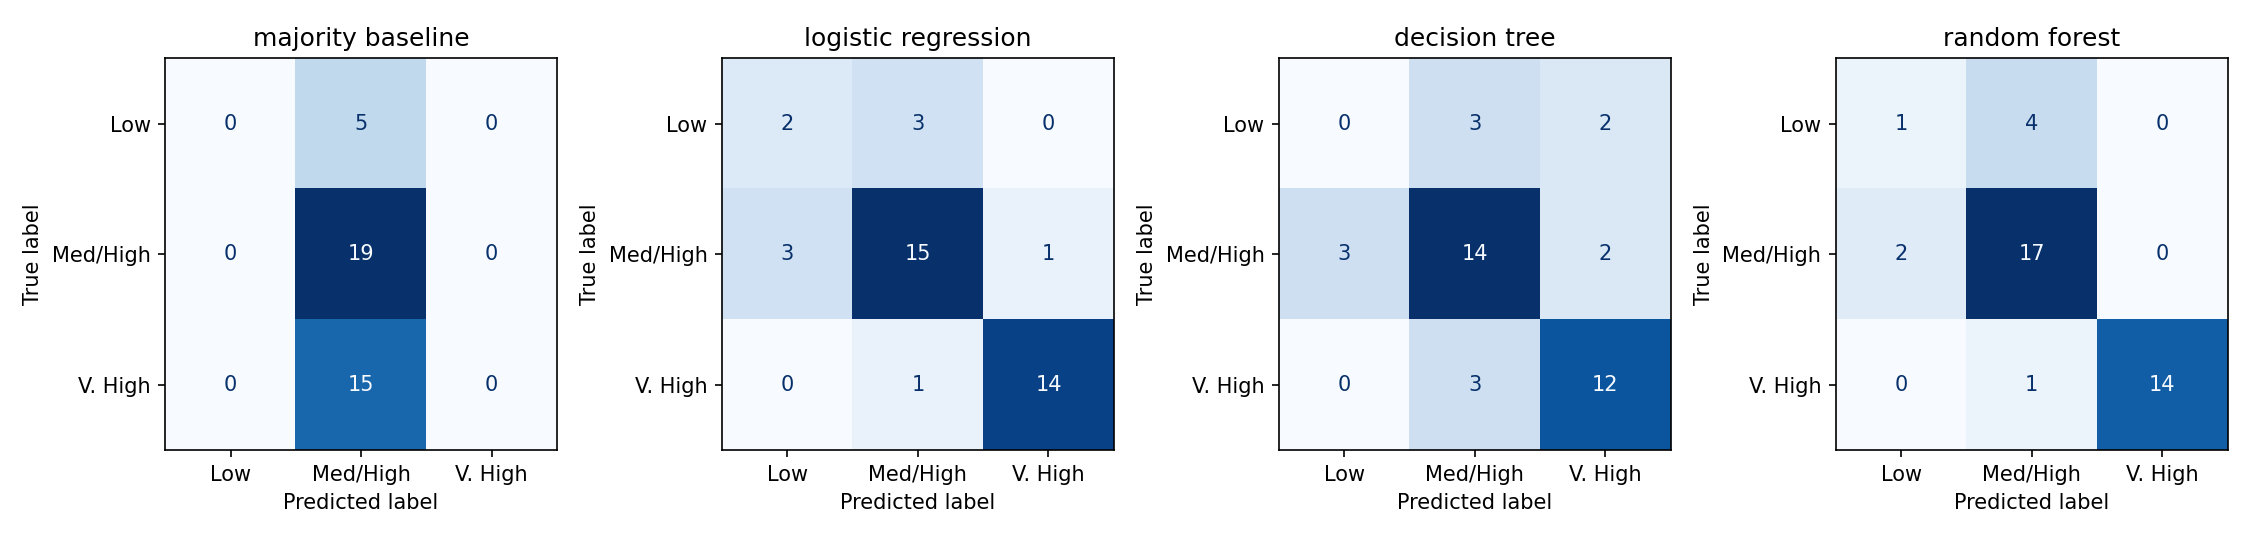
\includegraphics[width=0.90\textwidth]{confusion_matrices.png}
\caption{Confusion matrices on the test set (rows: true class; columns: predicted class).}
\label{fig:cm}
\end{figure}

Almost all errors are between neighbouring classes (Figure~\ref{fig:cm}). Logistic regression and the random
forest never confuse Low with Very High; the decision tree puts two Low countries in Very High. Six of the random
forest's seven errors are countries with an HDI between 0.503 and 0.582, near the 0.550 threshold. Eritrea, Sudan,
Djibouti and Gambia are Low but were predicted Medium/High, and Tanzania (0.555) and Uganda (0.582) were predicted
Low. The only Very High error is Saint Kitts and Nevis (0.840). Countries this close to a cut-off look like the
neighbouring class in their indicators, so the hard threshold explains these errors as much as the model does.

\subsection{Which features matter}
We computed permutation importance for the random forest out of fold on the training and validation data, because
the test set has only five Low countries. Permuting electricity access lowers macro F1 by 0.171, infant mortality
by 0.096, internet use by 0.073 and the agriculture share by 0.048. Region accounts for 0.026, and
\code{DominantSector}, unemployment, industry, growth, inflation and trade for 0.010 or less each. The logistic
regression coefficients, on standardised features, agree: higher infant mortality raises the Low score ($+3.01$)
and strongly lowers the Very High score ($-5.28$), the agriculture share behaves in the same way, and internet use
raises the Very High score ($+3.61$). Because these predictors are highly correlated and the model is nearly
unregularised, the split of weight among them is unstable, so single coefficients are not separate effects. The
correlation also lowers permutation importance, as the forest can partly fall back on a correlated feature.

\subsection{Limitations}
Only 26 countries are Low and 5 of them are in the test set, so one country moves Low-class recall by 20 points. We
used stratified splits, macro F1 and balanced accuracy for this reason; class weighting is left for future work.
With 193 countries, the cross-validation standard deviations (0.07 to 0.09) are as large as the gaps between
models. Missing values are concentrated in the poorest countries, where mean imputation moves them towards the
sample average and may blur the Low class. Nineteen values come from 2021 or 2022 while the HDI is for 2023, and
annual figures such as Sudan's GDP growth of $-29\%$ capture short-run shocks more than long-run development.
Finally, the results are associations. Electricity access and low infant mortality predict a high HDI, but both
are also outcomes of development and are correlated with the excluded income and education components, so
changing one indicator would not necessarily change a country's class.

\subsection{Conclusion}
Electricity access, infant mortality, internet use and the agriculture share of GDP are enough to place most
countries in the correct category. Logistic regression and the random forest reach 79\% and 82\% test accuracy,
against 49\% for the majority baseline, with cross-validated macro F1 between 0.85 and 0.90. Region, the engineered
sector feature and PCA add little to these four indicators. The Low class is the hardest to predict. It has only 26
countries and the most missing data, and 12 of them have an HDI within 0.05 of the 0.550 threshold.

\end{document}
